\begingroup

\TPGrid{3}{36}
\textblockorigin{0mm}{0mm}
\setlength{\parindent}{0mm}
\setlength{\banderougewidth}{2\TPHorizModule}
\setlength{\banderougeheight}{\TPVertModule}
\setlength{\bandeorwidth}{\TPHorizModule}
\setlength{\bandeorheight}{\banderougeheight}
\setlength{\imageheight}{29\TPVertModule}
\setlength{\imagewidth}{3\TPHorizModule}
\setlength{\logoheight}{2.5\TPVertModule}
\setlength{\gapwidth}{0.75pt}
\addtolength{\bandeorwidth}{-\gapwidth}
\addtolength{\imageheight}{-\gapwidth}

\begin{frame}[plain]
  %% UL banner
  \begin{textblock*}{3\TPHorizModule}[0,1](0mm,30\TPVertModule)
    \textcolor{rouge}{\rule{\banderougewidth}{\banderougeheight}}% % red stripe
    \rule{\gapwidth}{0pt}%                                         % gap
    \textcolor{or}{\rule{\bandeorwidth}{\bandeorheight}}           % gold stripe
  \end{textblock*}

  %% UL logo
  \begin{textblock*}{\TPHorizModule}(2\TPHorizModule,31\TPVertModule)
    \rule{\gapwidth}{0pt}%                                     % gap
    \includegraphics[height=\logoheight,keepaspectratio=true]{ul_p}
  \end{textblock*}

  %% background image
  \begin{textblock*}{3\TPHorizModule}(0mm,0mm)
    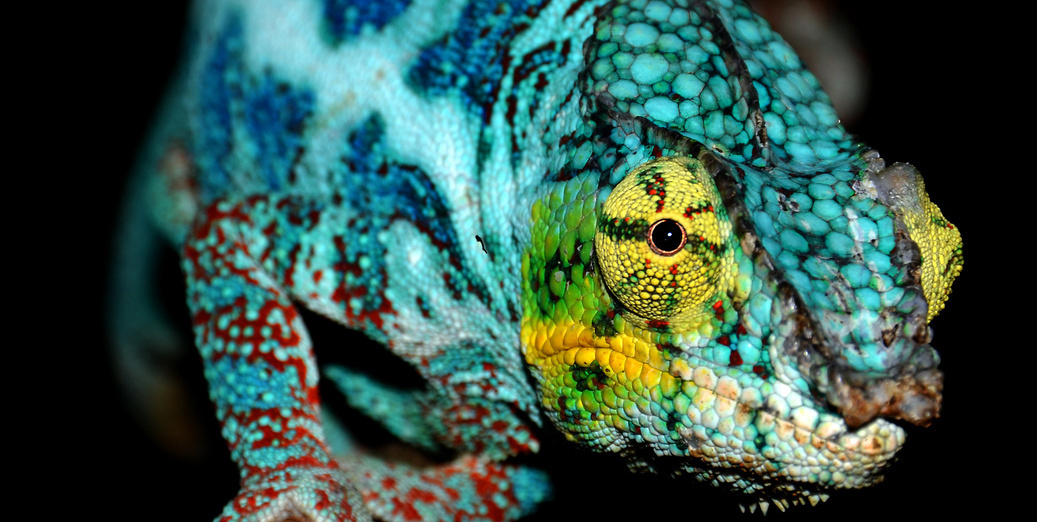
\includegraphics[height=\imageheight,width=\imagewidth]{furcifer-pardalis-nosy-faly}
  \end{textblock*}

  %% title
  \begin{textblock*}{2\TPHorizModule}(0.205\TPHorizModule,3.1\TPVertModule)
    %% Poor Man's (but simple!) shadow effect behind letters; needed
    %% to let the title stand out on the dark background
    \raggedright%
    \bfseries
    \fontsize{20}{20}\selectfont
    \textcolor{black}{%
      The Best of Both Worlds: \\
      Using Blended Learning \\
      in Actuarial Science Courses} \\
    \mdseries
    \fontsize{14}{18}\selectfont
    \textcolor{black}{Actuarial Teaching Conference 2017}
  \end{textblock*}
  \begin{textblock*}{2\TPHorizModule}(0.2\TPHorizModule,3\TPVertModule)
    \raggedright%
    \bfseries
    \fontsize{20}{20}\selectfont
    \textcolor{white}{%
      The Best of Both Worlds: \\
      Using Blended Learning \\
      in Actuarial Science Courses} \\
    \mdseries
    \fontsize{14}{18}\selectfont
    \textcolor{white}{Actuarial Teaching Conference 2017}
  \end{textblock*}

  %% date
  \begin{textblock*}{2\TPHorizModule}(0.2\TPHorizModule,26\TPVertModule)
    \fontsize{10}{12}\selectfont
    \textcolor{white}{June 27, 2017}
  \end{textblock*}
\end{frame}
\endgroup

%%% Local Variables:
%%% mode: latex
%%% TeX-engine: xetex
%%% TeX-master: "ATC2017-blended-learning"
%%% End:
